\chapter{Preâmbulo Teórico}

Para que possamos fazer uma análise comparativa entre duas estratégias estatísticas, temos que, antes, entender suas diferenças e similaridades, bem como as características dos dados com os quais estamos lidando.

Assim, este capítulo será dividido em duas grandes seções, uma destinada à apresentação das bases de imagens utilizadas, outra destinada à discussão sobre as qualidades dos dados nessas bases.

\section{As bases de dados}\label{sec:imdb}

Para o cumprimento desse trabalho, escolhemos duas bases de imagens diferentes, que chamaremos simplesmente Toyama e LIVE.

A base Toyama é, na verdade, chamada \textbf{IRCCyN/IVC-Toyama database (LCD)} e tem acesso franqueado no site ~\cite{Tourancheau2008} do IRCCyN (\emph{Institut de Recherche en Communications et Cybernétique de Nantes}), da Universidade de Nantes, na França.

A base LIVE é, na verdade, chamada \textbf{LIVE Image Quality Assessment Database} e tem acesso também franqueado no site ~\cite{livedb} do LIVE (\emph{Laboratory for Image \& Video Engineering}). Utilizamos sua \emph{release 1} nesse trabalho, por ser a única que disponibilizava dados de avaliação subjetiva para compressão JPEG.

Ambas as bases possuem imagens originais (não degradadas) e um determinado número de imagens degradadas com diferentes tipos e graus de degradação; nosso trabalho se concentra na degradação do tipo JPEG, em todos os graus de degradação disponíveis nas bases. A Tabela \ref{tab:bds} apresenta as principais características de ambas as bases. 

\begin{table}[htb]
	\footnotesize
	\caption[Características das Imagens das Bases de Dados]{Características das Imagens das Bases de Dados}
	\label{tab:bds}
	\centering
 	\begin{tabular}{ l | c | c } %\toprule[1.5pt]
% \begin{minipage}{\linewidth}
% 	\captionof{table}{Características das Imagens nas Bases de Dados} \label{tab:bds}
% 	\begin{tabular}{ l | c | c } %\toprule[1.5pt]
							&	\textbf{Toyama}			&	\textbf{LIVE} 		\\\hline % \midrule
		Número Total de Imagens	$T_i$		&	$98$				&	$204$	  		\\ % \midrule
		Número de Imagens de Referência $I_r$	& 	$14$				&	$29$		  	\\
		Número de Imagens degradadas $I_d$	&	$84$				&	$175$	  		\\
		Resolução das Imagens na base		& 	$768 \times 512$ pixels 		&	$768 \times 512$ pixels 	\\
		Profundidade de cor			&	$24bits/pixel$			&	$24bits/pixel$ 		\\
		Formato das imagens cedidas		&	BMP				&	BMP		  	\\
		Tipo de degradação			&	JPEG				&	JPEG		  	\\
		Graus de degradação aplicados		& $15$, $20$, $27$, $37$, $55$, $79$ 	& 	não informado 		\\
		Diversidade de graus de degradação	&	$6$ taxas			&  	não informado 		\\
		Faixa de valores de avaliação		& 	$[1, 5]$			& 	$[0, 100]$		\\
		Categorias de Qualidade			&	$5$				& 	$5$			\\
		Sessões de Avaliação distintas		&	$1$				& 	$2$			\\
		
%		\bottomrule[1.25pt]
	\end {tabular}\par
	\legend{Fontes: \cite{livedb,Tourancheau2008}}
\end{table}

As \autoref{fig:liveref} e \autoref{fig:livedist} apresentam exemplos de figuras disponíveis na base LIVE; já as figuras \autoref{fig:toyaref} e \autoref{fig:toyadist} provém da base Toyama. As imagens à esquerda são imagens de referência, não-corrompidas, enquanto as da direita já passaram pela compressão JPEG.

\begin{figure}[htb]
 \label{fig:liveex}
 \centering
  \begin{minipage}{0.48\textwidth}
    \centering
    \caption{Imagem de referência LIVE} \label{fig:liveref}
    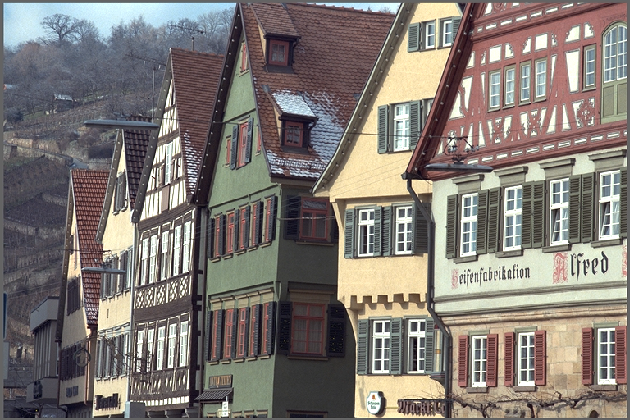
\includegraphics[width=\textwidth]{../img/liveref66.pdf}
    \legend{Fonte: \cite{livedb}}
  \end{minipage}
  \hfill
  \begin{minipage}{0.48\textwidth}
    \centering
    \caption{Imagem distorcida LIVE} \label{fig:livedist}
    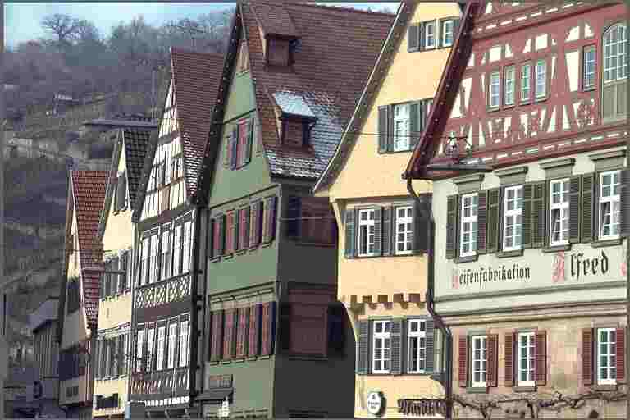
\includegraphics[width=\textwidth]{../img/liveref90.pdf}
    \legend{Fonte: \cite{livedb}}
  \end{minipage}
\end{figure}

Segundo a LIVE, o estudo que gerou as bases conduziu duas sessões de avaliação distintas. Os pesquisadores tiveram o cuidado de apresentar, em ambas as sessões, todas as imagens de referência e suas respectivas distorções. A quantidade de sujeitos no experimento foi diferente em cada sessão: na primeira, houve vinte sujeitos, na segunda, apenas treze. Os pesquisadores afirmam que a escolha das imagens para o estudo foi tal que possibilitaria uma distribuição aproximadamente uniforme das notas de avaliação, o que pode ser visualizado no histograma da \autoref{graf:liveHist}. Não foi imposta restrição de distância de visualização para a avaliação e as imagens foram mostradas aos sujeitos aleatoriamente. Para emitir suas opiniões, os sujeitos poderiam levar o tempo que necessitassem, mas só poderiam visualizar cada imagem apenas uma vez. Os pesquisadores promoveram uma pequena sessão de treinamento antes do início de cada sessão de avaliação. Estas informações e maiores detalhes podem ser obtidos no \emph{site} da referida base.

\begin{figure}[htb]
%	\label{graf:liveHist}
	\centering
	\begin{minipage}{.8\textwidth}
		\centering
		\caption{Histograma de avaliação subjetiva  --- LIVE}\label{graf:liveHist}
		\includegraphics{../../graphs/L_Hist_OSs.pdf}
		\legend{Histograma gerado a partir das opiniões dos sujeitos sobre a totalidade das imagens da base}
	\end{minipage}
\end{figure}

\begin{figure}[htb]
 \label{fig:toyaex}
 \centering
  \begin{minipage}{0.48\textwidth}
    \centering
    \caption{Imagem de referência Toyama} \label{fig:toyaref}
    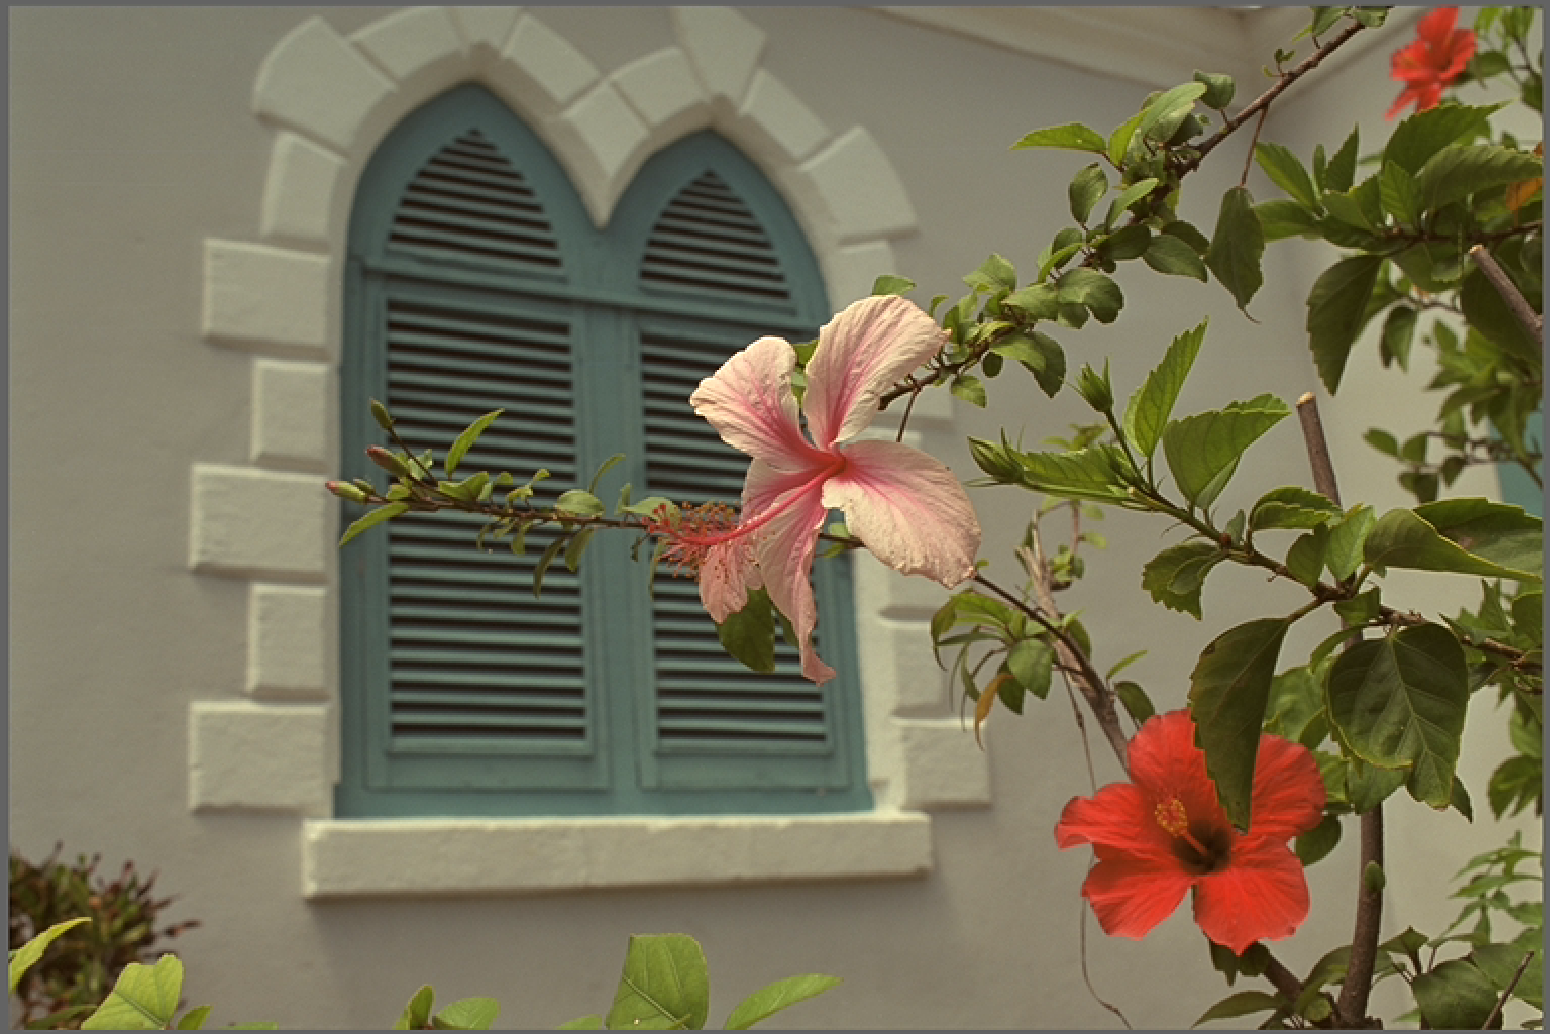
\includegraphics[width=\textwidth]{../img/toyaref07.pdf}
    \legend{Fonte: \cite{Tourancheau2008}}
  \end{minipage}
  \hfill
  \begin{minipage}{0.48\textwidth}
    \centering
    \caption{Imagem distorcida Toyama} \label{fig:toyadist}
    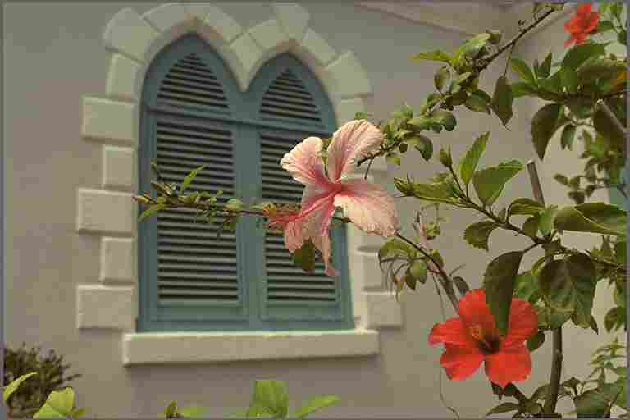
\includegraphics[width=\textwidth]{../img/toyadist07_79.pdf}
    \legend{Fonte: \cite{Tourancheau2008}}
  \end{minipage}
\end{figure}

Segundo o arquivo de informações que acompanha a base Toyama, foram dezesseis não-peritos que avaliaram as imagens dessa base, em sua maioria estudantes, não informando se houve ou não sessões distintas. Da mesma forma que a LIVE, as imagens foram apresentadas aleatoriamente, sem restrição de tempo e também com apenas uma oportunidade de avaliação para cada imagem. Neste estudo foi imposta a distância de observação igual a quatro vezes a altura da imagem. A Toyama apresenta dezesseis avaliações distintas para cada imagem, totalizando, portanto, dezesseis sujeitos no experimento. O histograma das notas de avaliação das imagens dessa base pode ser observado na \autoref{graf:toyaHist}.
 

\begin{figure}[htb]
%	\label{graf:liveHist}
	\centering
	\begin{minipage}{.8\textwidth}
		\centering
		\caption{Histograma de avaliação subjetiva --- Toyama}\label{graf:toyaHist}
		\includegraphics{../../graphs/T_Hist_OSs.pdf}
		\legend{Histograma gerado a partir das opiniões dos sujeitos sobre a totalidade das imagens da base}
	\end{minipage}
\end{figure}

Ambas os grupos de pesquisa deram a seus sujeitos uma escala com as palavras ``\emph{bad}'', ``\emph{poor}'', ``\emph{fair}'', ``\emph{good}'' e ``\emph{excellent}'', mas cada uma associou a essas palavras uma escala diferente. Além de os intervalos de avaliação serem distintos, como pode ser observado na \autoref{tab:bds}, outra diferença se faz digna de nota: a LIVE considera contínuo e linear o domínio de avaliação, enquanto a Toyama considera esse domínio discreto. Ou seja, na LIVE encontraremos notas como $4,55$, ou $9,42$ e na Toyama, apenas os inteiros entre $[1,5]$. A Toyama ainda informa que seus testes foram executados conforme as condições de avaliação apontadas no ITU-R Rec. 500-10. Veremos mais detalhes sobre essa recomendação, e outras, na sessão seguinte.

\section{Avaliação de Qualidade de Imagens}

Como dito no \autoref{chap:intro}, os atuais usos de imagens e vídeos digitais têm sua abrangência amplificada, na medida em que novos serviços surgem no mercado --- e que mais usuários utilizam esses serviços. Isso, como dito, se torna um desafio pra indústria, que precisa encontrar formas cada vez mais econômicas e eficientes de entregar seus produtos (mídias digitais) utilizando a infra-estrutura de comunicação existente e com o mínimo custo computacional e de armazenamento.

Para resolver problemas de armazenamento e tráfego, algoritmos de compressão foram desenvolvidos e são utilizados corriqueiramente. Padrões como o JPEG e MPEG são muito frequentemente utilizados por pessoas que desejam assistir vídeos online ou trasmitir fotos pelo celular. Alguns dos algoritmos utilizados hoje em dia são classificados como ``sem perdas'' (PNG e TIFF são alguns exemplos), o que significa que, uma vez descompactas, as imagens resultantes guardam as mesmas características das images originais --- o mesmo volume de dados dentro da mesma conformação espacial. Outros algoritmos, que consideram a perda de informação como razoável, são considerados ``com perdas'', e atingem taxas de compressão mais elevadas. Exemplos de algoritmos com perdas são os já citados JPG (imagem) e MPEG (vídeo).

Estabelece-se então uma relação de compromisso entre compactação (com perda de informação) e qualidade, já que é mais interessante para a indústria assumir um percentual de perda em benefício de economia de espaço e banda de tráfego. Contudo, junto com a perda de informação caminha a perda de qualidade. 

Qual o mínimo de informação para que, aferindo economia, mantenha-se a mesma qualidade percebida no produto final? Nesse contexto se situa o campo de pesquisa em qualidade de imagem. E como aferir essa qualidade? Atualmente, encontra-se duas formas distintas e dependentes: o método subjetivo de aferição de qualidade e o objetivo.

O método subjetivo ainda é o mais confiável, pois se basea na aferição a partir de observadores humanos. À pessoas são apresentadas imagens, cujas qualidades são eferidas e anotadas. Afinal, nada melhor do que o próprio cliente aferindo a qualidade do produto entregue. Essa abordagem, contudo tem algumas restrições.

A primeira grande restrição é a econômica. Para que a aferição seja feita por seres humanos é necessário que esses sujeitos sejam contratados, ou que se aloque recursos para que o material chegue até pessoas dispostas a fazer essa aferição gratuitamente. O segundo grande custo é o tempo: aferições humanas dependem de logística e tempo de processamento dos dados obtidos.

Para que se tenha uma opinião considerada estatisticamente relevante para uma população, é necessário um grande número de sessões de avaliação, com uma gama de indivíduos bastante diversa --- idealmente diversa a ponto de representar uniformemente todas as variâncias da população em questão. Essa consideração reforça as restrições de tempo e de custo financeiro. Esse tipo de avaliação é raramente executada com indivíduos ou imagens suficientes para que se possa fazer inferências a respeito do público em geral. Como dito na seção anterior (\autoref{sec:imdb}), as bases com as quais trabalhamos, largamente conhecidas e exploradas nas literaturas da área, tem poucas imagens e ainda menos avaliações. Portanto, inferências para uma população são inviáveis a partir dessas observações --- que servem apenas para fins acadêmicos.

Problemas que podem ser encontrados em estudos estatísticos são os chamados ``\emph{bias}'', que podem ser inseridos no estudo a partir da amostragem indevida da população para participação nos testes~\cite{boslaugh2008}, ainda na fase de design de tais testes. Esse tipo de consideração deve ser feita sobre as imagens que analisamos, já que estudos demonstram que ``experts'' na área de qualidade visual tentem a ser mais criteriosos em suas avaliações de qualidade; principalmente por já saberem o que procurar, no que tange erros e distribuição espacial destes. Apesar de a Toyama alegar que seus sujeitos são não-peritos, ela também alega que são estudantes de nível superior, e que, portanto, não representam bem a população de possíveis consumidores de imagens, que podem ter não só níveis diversos de educação formal como também podem ter qualquer idade.

A LIVE alega promover uma pequena sessão de treinamento antes da sessão de avaliação, mas não dá características dessas sessões. Veremos a seguir, como a forma de se colocar uma pergunta pode influenciar na resposta obtida e, portanto, questionar essa sessão prévia de treinamento é completamente válido.

Por conta dessa grande diversidade de fatores que influenciam a avaliação de qualidade de uma imagem e a validade estatística dos resultados, foram criados padrões de teste, que foram normatizados pelo ITU. Alguns exemplos são:

\begin{description}
	\item{As referências que eu tenho são todas sobre video.} Quais posso encontrar sobre imagens? Deveria consultar os padrões?
\end{description}

O método de avaliação subjetiva ainda é o \emph{benchmark} contra o qual todos os métodos objetivos são comparados. Em nosso estudo, seguindo as tendências da área, apresentamos gráficos \textbf{métrica vs. MOS}.

Por conta dessa característica humana, esse tipo de avaliação é intrinsecamente estatística, e tem sido tratada como tal. A forma desse tratamento estatístico será alvo de maiores discussões nesse trabalho.

A alternativa que surge aos métodos subjetivos é a confecção de algoritmos e estratégias computacionais que possam aferir e indicar a qualidade de uma imagem automaticamente. Claramente, uma imagem não tem para um sistema computacional o mesmo significado que tem para humanos. Nós tendemos a avaliar conteúdo e estrutura, reconhecer uma paisagem ou uma pessoa. Existem informações semânticas em imagens que fazem sentido apenas para humanos. Dessa forma, devemos buscar formas que um computador possa aferir a diferença entre duas imagens, ou buscar estrutura nelas.

As estratégias para extração de conteúdo de uma imagem podem ser distribuídas em três grupos:

\begin{description}
	\item{avaliação baseada em pixels:}
		Os métodos de extração de informação desse grupo advém principalmente de outras áreas de processamento de sinais e são razoavelmente bem conhecidas nas engenharias como um todo: MSE (\emph{Mean Square Error}, Erro Quadrático Médio) e PSNR (\emph{Peak Signal-to-Noise Ratio}, Razão de Pico Sinal-Ruído). Dentro da área de avaliação de qualidade visual, foi desenvolvida uma outra métrica em anos recentes, a MSSIM (\emph{Mean Structural Similarity Index}, Média de Índice de Similaridade Estrutural), que ganhou relevante destaque em publicações da área, apesar de sua eficiência controversa.
\end{description}
Com aferir a qualidade de uma imagem? O assunto é extenso e complexo e passa por definir o que é, de fato, qualidade. Vários fatores influenciam na avaliação da qualidade por humanos, como já dito. Uma pessoa que tenha uma conexão emocional com uma paisagem tende a atribuir maior qualidade a uma imagem que contenha a paisagem em questão. Trilhas sonoras e sincronização de áudio (especialmente no caso de fala e sincronização labial) tendem a influenciar a avaliação de qualidade de um trecho de vídeo \cite{Winkler-2005-Wiley}. Avaliações humanas são intrínsecamente estatísticas e uma boa indicação de qualidade subjetiva é a MOS (\emph{Mean Opinion Score}, inglês para ``Pontuação Média de Opinião'').

Além da avaliação humana, existem esforços para a criação de sistemas de avaliação objetiva de imagens,Existem avaliações subjetivas e objetivas. Avaliações subjetivas são feitas apresentando imagens a humanos, que as avaliam em qualidade. Muitos fatores influenciam nessa avaliação subjetiva de imagens ou vídeo, um exemplo interessante é a influência da trilha sonora na percepção de qualidade de vídeo \cite{Winkler-2005-Wiley}. Avaliações objetivas são feitas a partir de sistemas computadorizados, algoritmos criados para esse fim. Infelizmente, a avaliação objetiva ainda está muito aquém do desejado~\cite{wang-bovik2006}. , a qualidade de imagens pode ser aferida objetiva e subjetivamente. Aferições subjetivas de qualidade são feitas segundo estratégias bem definidas

O autor de \cite{Winkler-2005-Wiley} 
